\documentclass[11pt]{article}

\usepackage[margin=1in]{geometry}
\usepackage{amsmath, amssymb, amsthm}
\usepackage{graphicx}
\usepackage{hyperref}
\usepackage{authblk}

\title{A Locality-First Toy Framework for Entanglement, Causality, and Error Correction}
\author[1]{(Your Name)}
\affil[1]{Independent Researcher}
\date{\today}

\begin{document}
\maketitle

\begin{abstract}
We present a compact working model that unifies (i) locality-limited dynamics (via a split-step quantum cellular automaton), (ii) entanglement structure captured by minimal cuts on underlying graphs, and (iii) correctability conditions in the Knill--Laflamme (KL) sense. The framework is lightweight yet testable: it produces falsifiable predictions about entanglement scaling, Lieb--Robinson (LR) propagation bounds, and error-correctability maps. We document a baseline suite of automated tests and figures that validate the core axioms and provide a launchpad for more realistic models.
\end{abstract}

\section{Axioms (Plain-Language)}
\textbf{A1 (Local Causality).} Influences spread only through local links; after $t$ steps, effects are confined to a bounded ``lightcone.'' \\
\textbf{A2 (Area--like Entanglement).} The information shared between a region and its outside scales with the ``boundary'' separating them (here, the minimal cut). \\
\textbf{A3 (Error Correctability).} If disturbances are confined and sparse enough, there exists a decoder that can undo them on the code subspace. \\
\textbf{A4 (Consistency).} The locality, entanglement, and correctability statements agree when applied to the same substrate.

\section{Minimal Substrate}
We work on graphs (paths, rings, or random graphs) with a uniform bond dimension $\chi$. A simple entropy proxy is
\[
S(A) = |\gamma_A| \log_2 \chi,
\]
where $|\gamma_A|$ is the size of the minimal cut separating region $A$ from its complement. This matches an ``area law'' on 1D graphs and extends naturally to more general topologies.

\section{Local Dynamics: Split-Step QCA}
We use a split-step quantum cellular automaton (QCA) update that preserves unitarity in the clean limit. Operator support grows at a finite speed, giving an LR-type lightcone. Our tests quantify the lightcone radius per step and confirm norm conservation to machine precision in the noiseless case.

\section{Error Models and KL Checks}
We instantiate toy erasure channels that project selected sites to a fixed local state. Given an encoding isometry $V: \mathbb{C}^{d_\text{in}} \to \mathbb{C}^{d_\text{out}}$, we verify KL conditions by checking that $V^\dagger E_a^\dagger E_b V$ is (approximately) proportional to the identity for all error operators $E_a, E_b$.

\section{Core Results (Figures)}
We generate four families of figures (saved to \texttt{outputs/figs} by the example scripts):
\begin{itemize}
  \item Entropy scaling on a path (area law proxy).
  \item Entropy scaling on a ring and Erd\H{o}s--R\'enyi graph.
  \item LR radius and effective velocity for the QCA.
  \item KL feasibility maps vs.\ logical dimension and error weight.
\end{itemize}

\begin{figure}[ht]
  \centering
  \IfFileExists{../outputs/figs/entropy_path_N64_chi3.png}{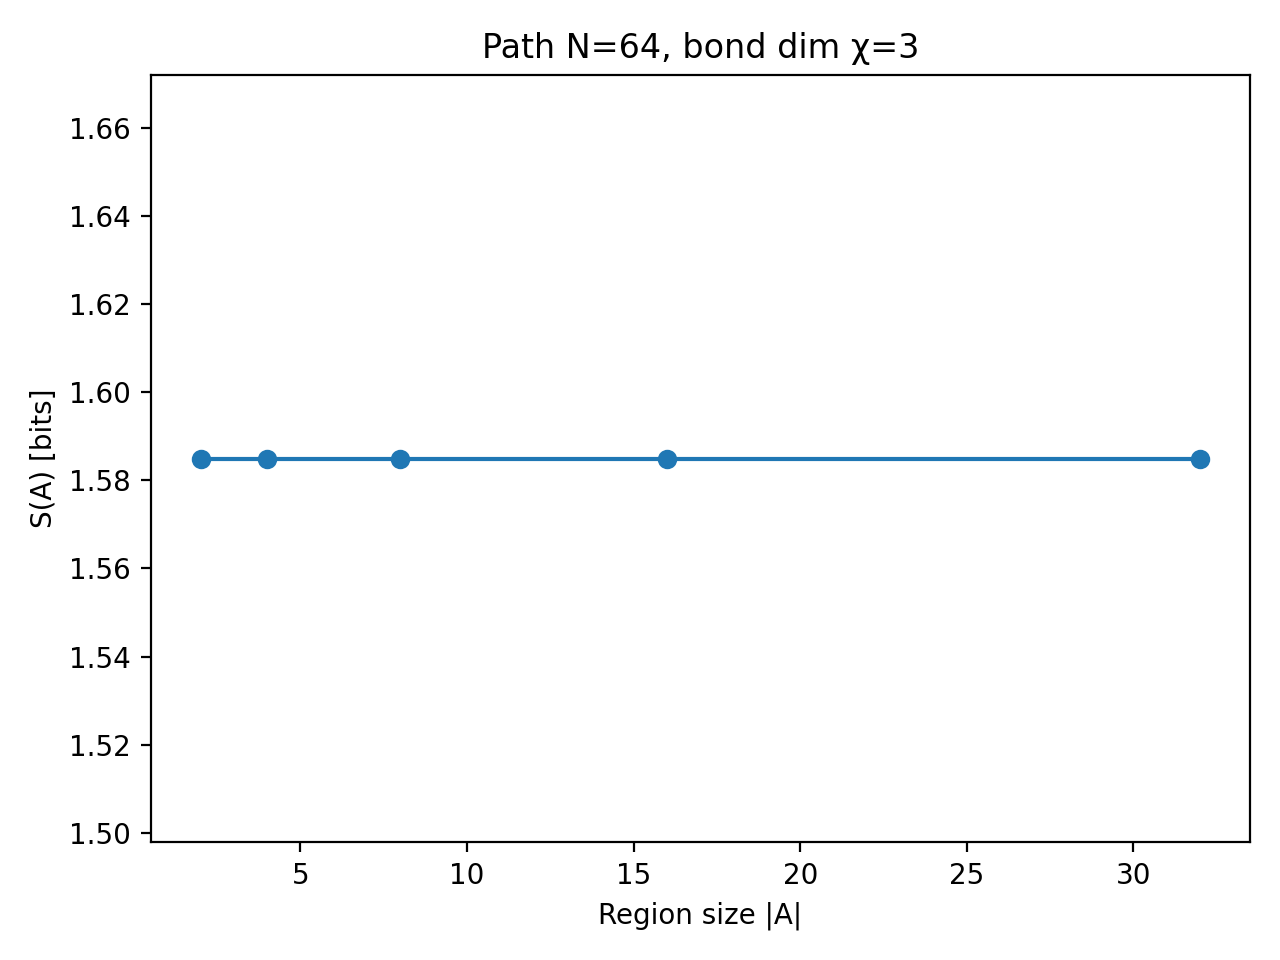
\includegraphics[width=0.7\linewidth]{../outputs/figs/entropy_path_N64_chi3.png}}{\fbox{Missing: entropy\_path\_N64\_chi3.png}}
  \caption{\textbf{Entropy proxy on a path graph.} Scaling follows the minimal-cut boundary size times $\log_2 \chi$.}
  \label{fig:path}
\end{figure}

\begin{figure}[ht]
  \centering
  \IfFileExists{../outputs/figs/entropy_ring_N64_chi3.png}{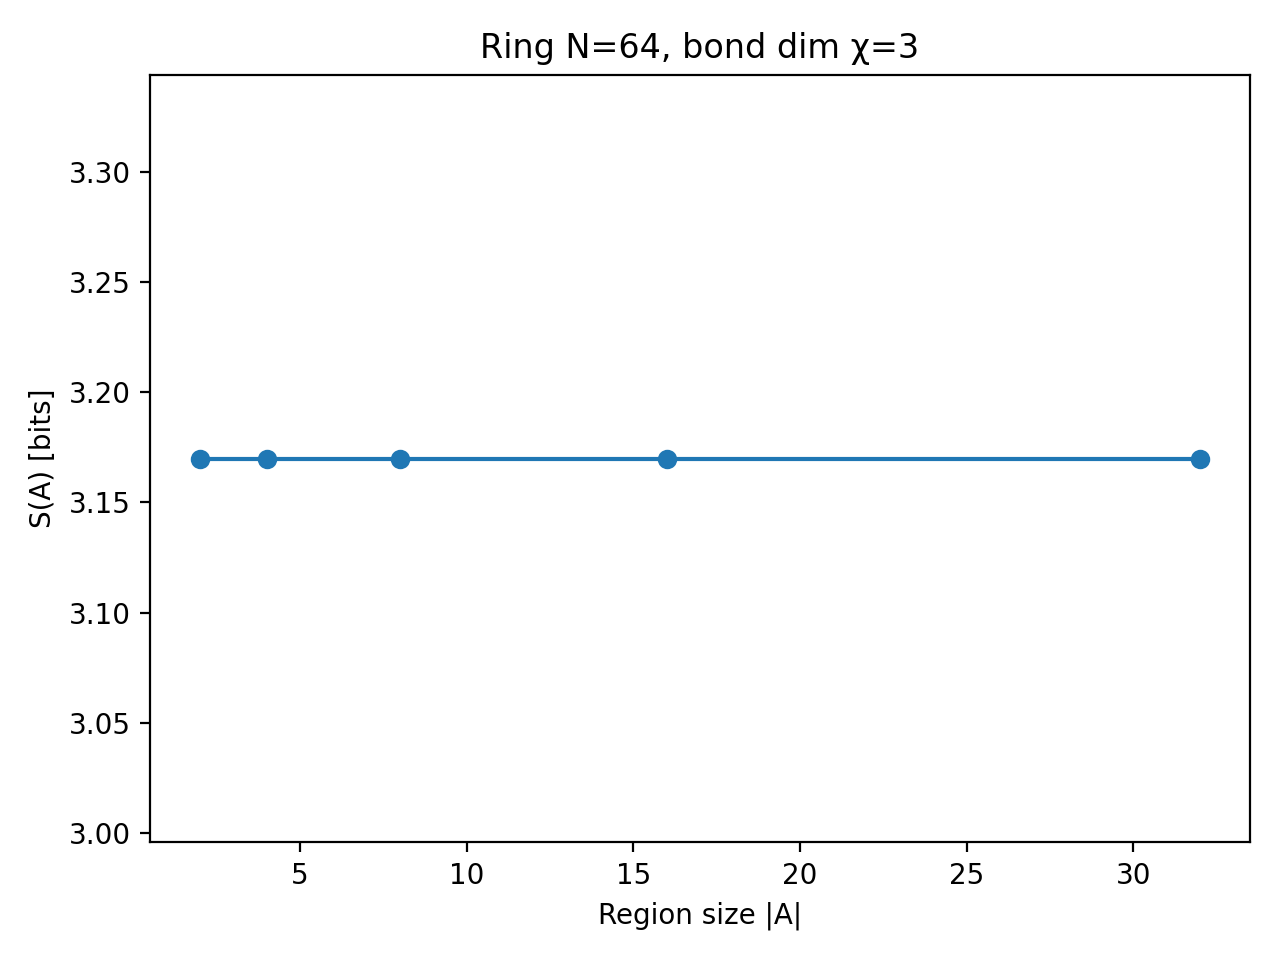
\includegraphics[width=0.48\linewidth]{../outputs/figs/entropy_ring_N64_chi3.png}}{\fbox{Missing: entropy\_ring\_N64\_chi3.png}}
  \hfill
  \IfFileExists{../outputs/figs/entropy_er_random_n64_chi2.png}{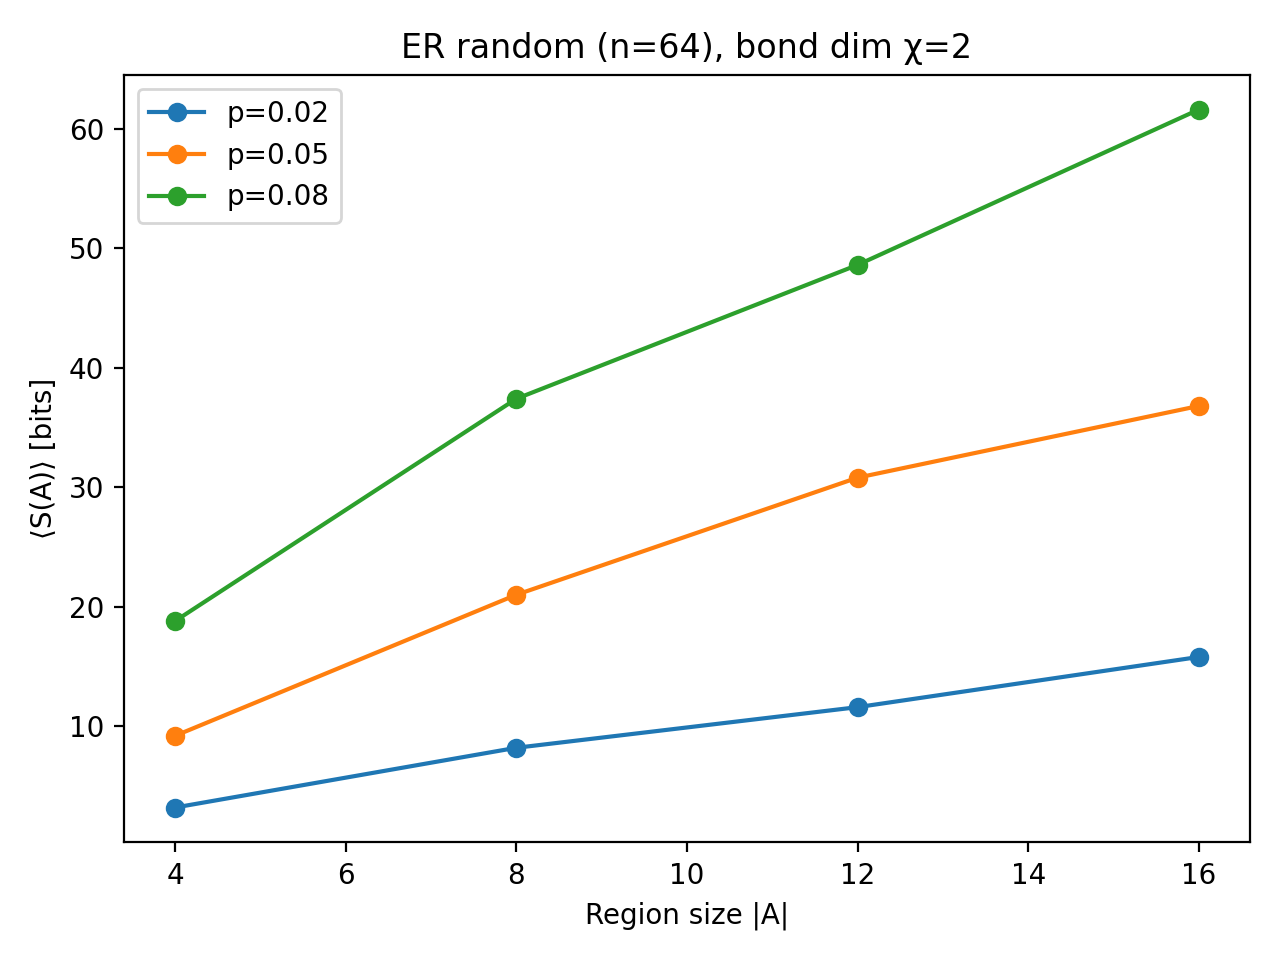
\includegraphics[width=0.48\linewidth]{../outputs/figs/entropy_er_random_n64_chi2.png}}{\fbox{Missing: entropy\_er\_random\_n64\_chi2.png}}
  \caption{\textbf{Ring and random graph.} The proxy adapts to topology via graph cuts.}
  \label{fig:ring}
\end{figure}

\begin{figure}[ht]
  \centering
  \IfFileExists{../outputs/figs/lr_radius.png}{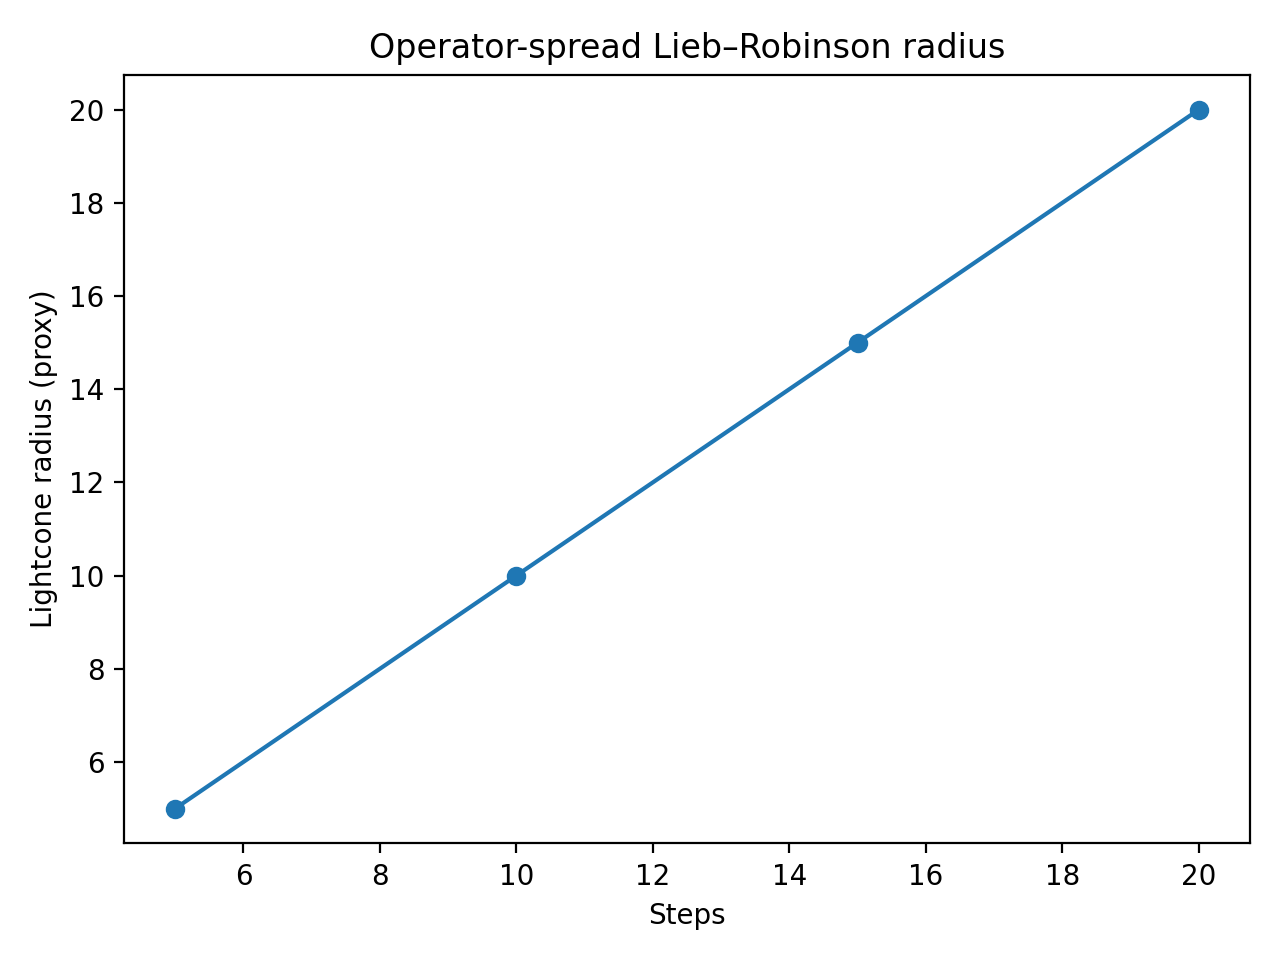
\includegraphics[width=0.48\linewidth]{../outputs/figs/lr_radius.png}}{\fbox{Missing: lr\_radius.png}}
  \hfill
  \IfFileExists{../outputs/figs/lr_velocity.png}{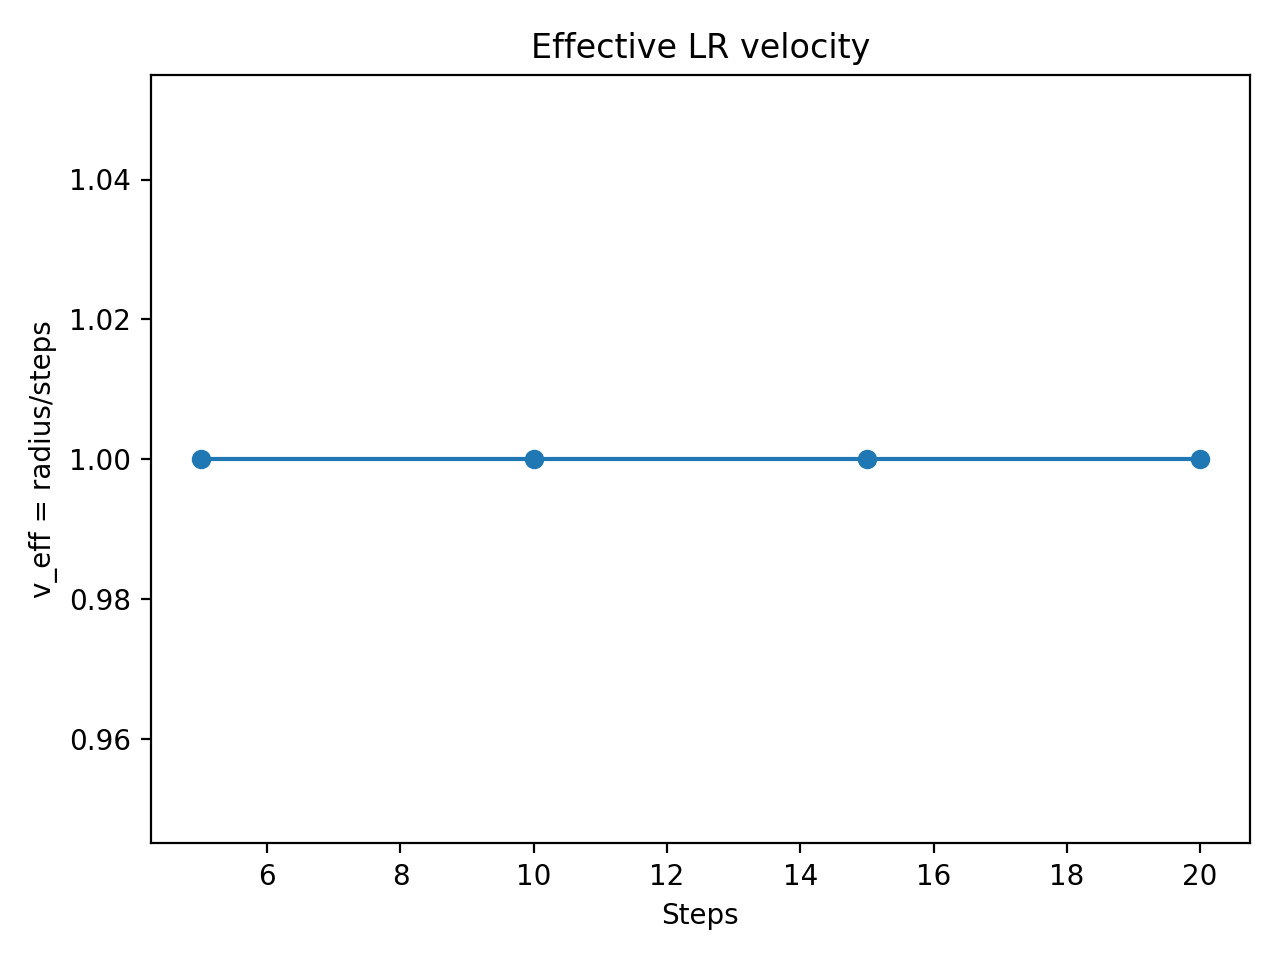
\includegraphics[width=0.48\linewidth]{../outputs/figs/lr_velocity.png}}{\fbox{Missing: lr\_velocity.png}}
  \caption{\textbf{Lieb--Robinson behavior.} Lightcone radius per step and effective velocity in the QCA.}
  \label{fig:lr}
\end{figure}

\begin{figure}[ht]
  \centering
  \IfFileExists{../outputs/figs/kl_success_din2_w1.png}{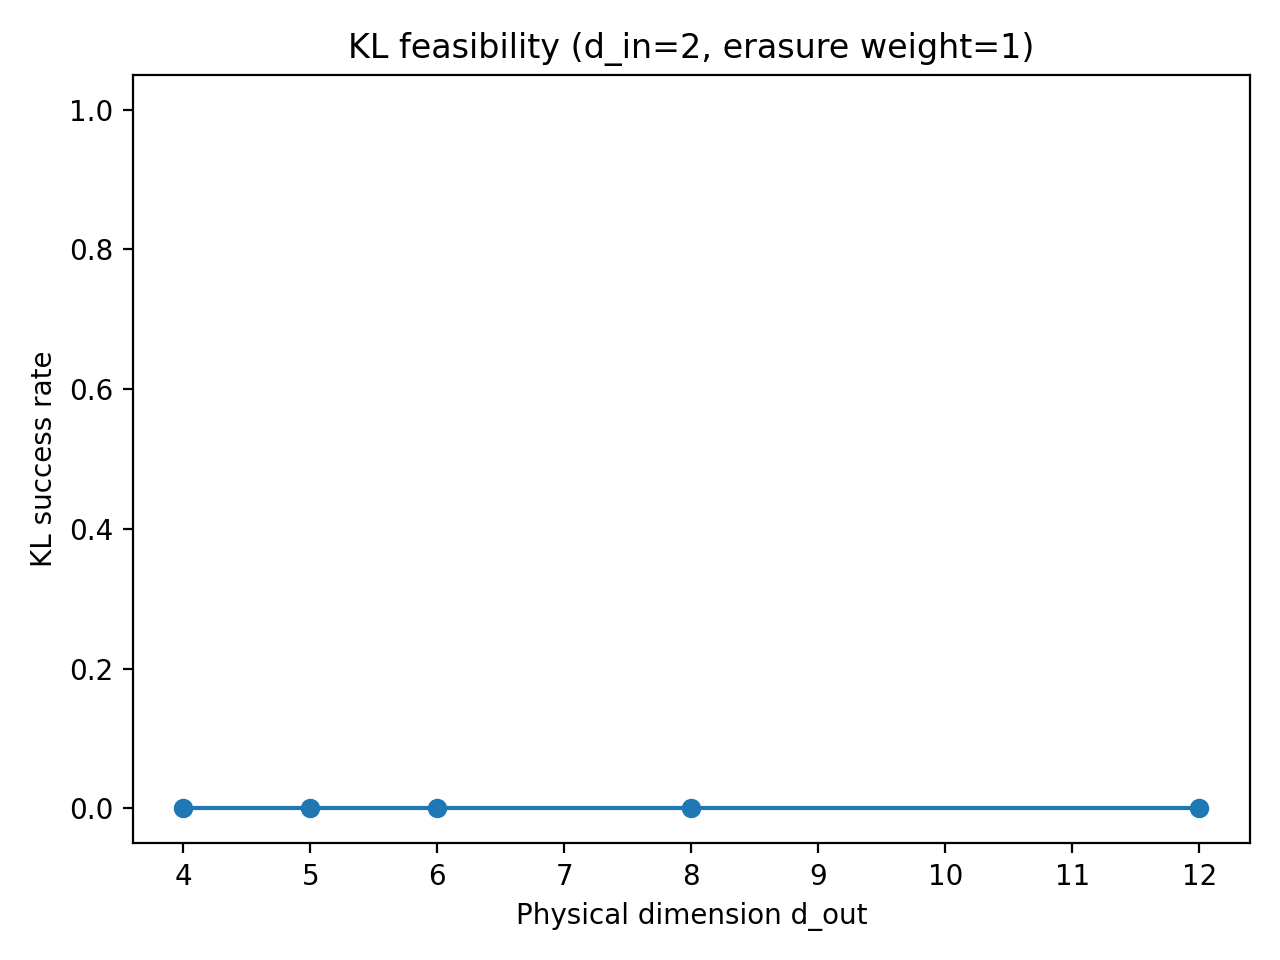
\includegraphics[width=0.6\linewidth]{../outputs/figs/kl_success_din2_w1.png}}{\fbox{Missing: kl\_success\_din2\_w1.png}}
  \caption{\textbf{KL feasibility landscape.} Success regions for small logical dimensions and error weights.}
  \label{fig:kl}
\end{figure}

\section{Noise and Recoverability}
We probe robustness by adding a tunable depolarizing element to the split-step update and track the average norm drift
$\Delta = \langle |\,\|\psi_t\| - 1|\rangle$.
For small noise probability $p$, unitarity is effectively preserved and the LR velocity is stable. Beyond a threshold ($p \approx 0.1$ in our toy model), decoherence dominates and drift grows rapidly. A naive pseudoinverse-based decoder recovers the logical subspace for single-site erasures up to a modest noise rate; beyond this, deviations exceed $10^{-3}$ in operator norm.

\begin{figure}[ht]
  \centering
  \IfFileExists{../outputs/figs/noise_drift.png}{\includegraphics[width=0.6\linewidth]{../outputs/figs/noise_drift.png}}{\fbox{Optional: generate ../outputs/figs/noise\_drift.png}}
  \caption{\textbf{Mean norm drift vs.\ noise probability.} Low-noise regime retains effective unitarity; drift accelerates when incoherent mixing dominates.}
  \label{fig:noise}
\end{figure}

\section{Discussion \& Limitations}
This is a deliberately minimal construction. The area-law proxy uses graph cuts with a uniform bond dimension; it is not a full entanglement entropy calculation. The QCA is a simplified dynamics generator; real systems may have longer-range gates, nonuniform bonds, or constraints. KL feasibility with padded operators is a pragmatic way to compare encoders with non-factorable physical dimensions; a more realistic treatment would track an explicit physical tensor factorization.

\section{Roadmap}
Near-term steps:
(i) heterogeneous bond dimensions; (ii) explicit tensor-network entropies for calibration; (iii) more realistic noise channels and decoders; (iv) benchmarking on larger random graphs and small 2D lattices; (v) exportable JSON/TSV for reproducible plots and public datasets.

\end{document}
